\documentclass[tikz,border=5pt]{standalone}
\usepackage[T1]{fontenc}
\usepackage{lmodern}
\usepackage{amsmath}
\usepackage{pgfplots}
\pgfplotsset{compat=1.18}

\definecolor{orblue}{RGB}{76,120,168}
\definecolor{ororange}{RGB}{209,143,0}
\definecolor{orgreen}{RGB}{80,140,90}
\definecolor{orred}{RGB}{178,80,80}
% Generated by scripts/create_manuscript_tables.py from outputs/runs/summarize-the-plot-of-hamlet-in-one-sentence/selection.json -- do not hand-edit.
\def\WorkedExampleTableRows{c0 & 0.606 & 1.00 & 0.20 & 38 & 0.486 \\
c1 & 0.387 & 1.00 & 0.20 & 32 & 0.327 \\
c2$^\ast$ & 0.644 & 1.00 & 0.20 & 33 & 0.574 \\
c3 & 0.575 & 1.00 & 0.20 & 38 & 0.455 \\
c4 & 0.288 & 1.00 & 0.20 & 33 & 0.218 \\}
\def\WorkedExampleWinner{c2}
\def\WorkedExampleQualityBars{(c0,0.6062) (c1,0.3875) (c2,0.6438) (c3,0.5750) (c4,0.2875)}
\def\WorkedExampleConfidenceBars{(c0,0.2000) (c1,0.2000) (c2,0.2000) (c3,0.2000) (c4,0.2000)}
\def\WorkedExampleConsistencyBars{(c0,0.0600) (c1,0.0600) (c2,0.0600) (c3,0.0600) (c4,0.0600)}
\def\WorkedExampleCostBars{(c0,-0.3800) (c1,-0.3200) (c2,-0.3300) (c3,-0.3800) (c4,-0.3300)}


\begin{document}
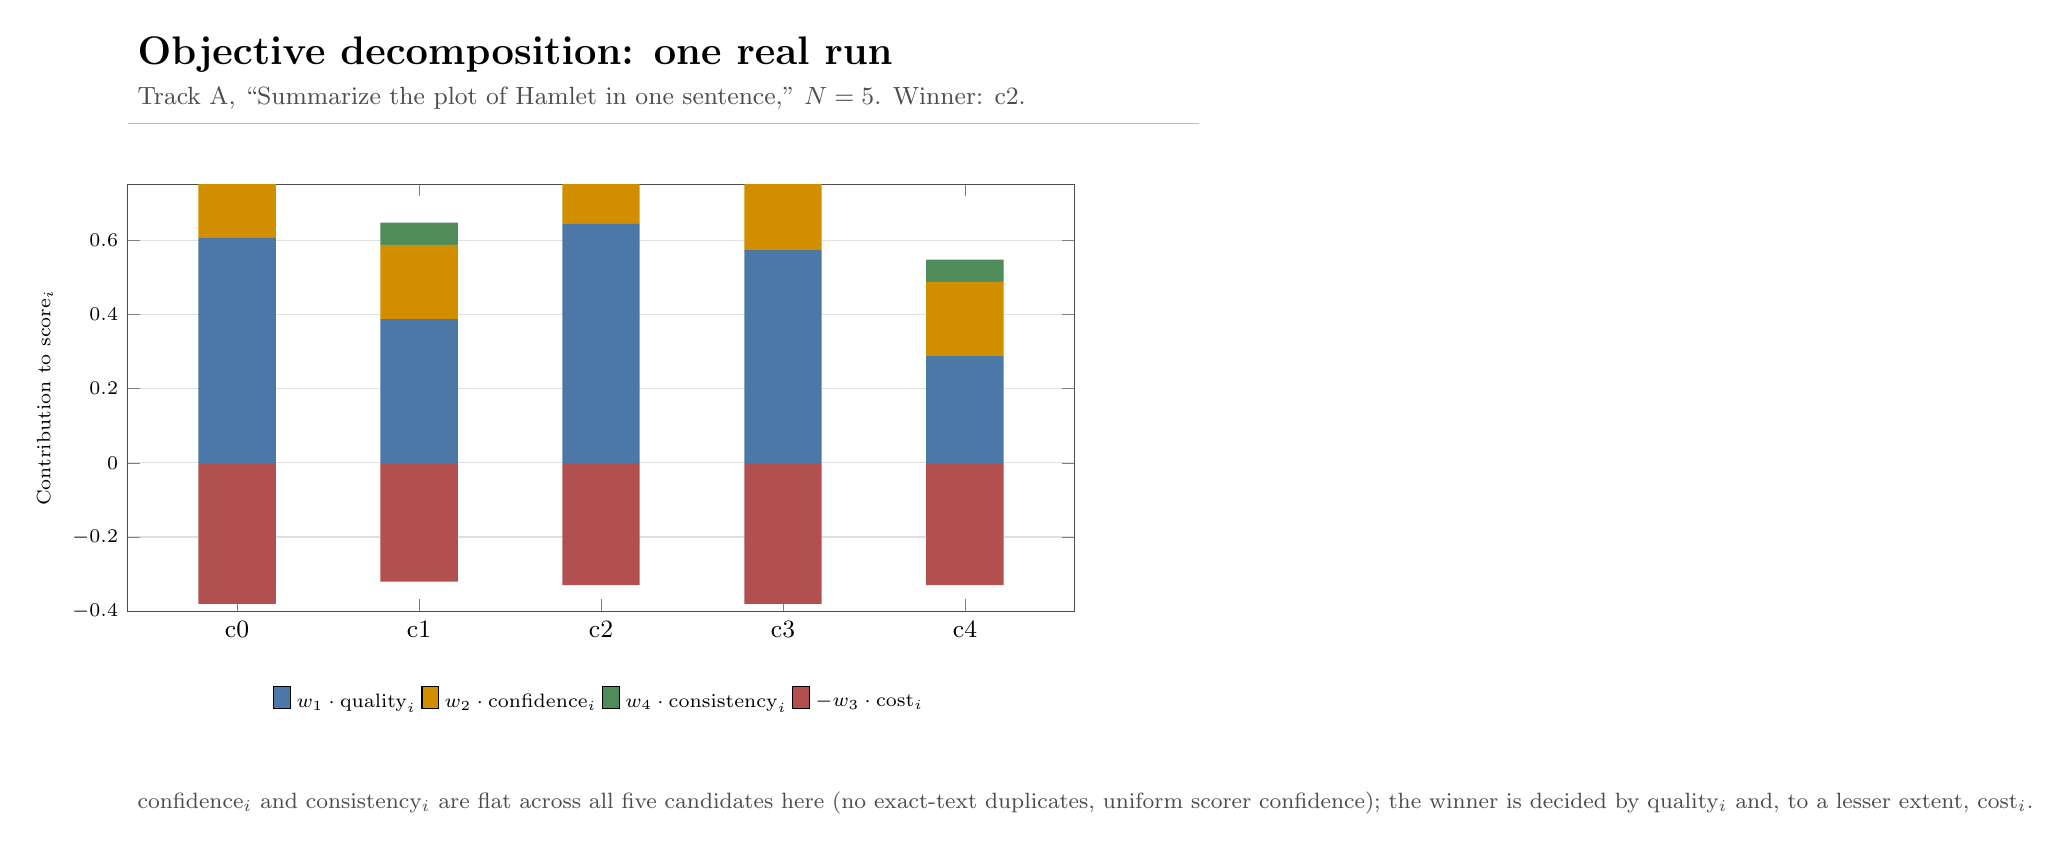
\begin{tikzpicture}
\node[anchor=west,font=\Large\bfseries] at (0,0) {Objective decomposition: one real run};
\node[anchor=west,font=\small,text=black!70] at (0,-0.55)
  {Track A, ``Summarize the plot of Hamlet in one sentence,'' $N=5$. Winner: c2.};
\draw[black!25] (0,-0.88) -- (13.6,-0.88);

\begin{scope}[yshift=-1.65cm]
\begin{axis}[
  at={(0,0)},anchor=north west,
  width=13.6cm,height=7.0cm,
  ybar stacked,bar width=28pt,
  ymin=-0.4,ymax=0.75,
  ylabel={Contribution to score$_i$},
  tick label style={font=\scriptsize},
  ylabel style={font=\scriptsize},
  symbolic x coords={c0,c1,c2,c3,c4},
  xtick=data,
  xticklabel style={font=\small},
  ymajorgrids=true,grid style={black!12},
  axis line style={black!70},
  enlarge x limits=0.15,
  legend style={at={(0.5,-0.16)},anchor=north,legend columns=4,font=\scriptsize,draw=none}
]
\addplot[fill=orblue,draw=none] coordinates {\WorkedExampleQualityBars};
\addlegendentry{$w_1\cdot\text{quality}_i$}
\addplot[fill=ororange,draw=none] coordinates {\WorkedExampleConfidenceBars};
\addlegendentry{$w_2\cdot\text{confidence}_i$}
\addplot[fill=orgreen,draw=none] coordinates {\WorkedExampleConsistencyBars};
\addlegendentry{$w_4\cdot\text{consistency}_i$}
\addplot[fill=orred,draw=none] coordinates {\WorkedExampleCostBars};
\addlegendentry{$-w_3\cdot\text{cost}_i$}
\end{axis}
\end{scope}

\node[anchor=west,font=\footnotesize,text=black!70] at (0,-9.5)
  {confidence$_i$ and consistency$_i$ are flat across all five candidates here (no exact-text duplicates,
  uniform scorer confidence); the winner is decided by quality$_i$ and, to a lesser extent, cost$_i$.};
\end{tikzpicture}
\end{document}
